%___________________________ Q 4.7 ______________________________
\subsection{Discuss how do you evaluate the performance of your control system and what are the limits of performance. (3 pts)}
\vspace{10pt}

%%Write your answer here

Our objective for this part of the course was to be able to control the position of the tip of a robotic arm. This came with some chalenges, the first one being that the object used to represent the arm, was a thin metal ruller that was not very rigid, meaning oscilation would happen whenever we moved, the second was the existance of dead zone in the motor and gearbox, this dead zone meant that for small values of the control signal the system would not react, meaning that the system would not reach the desired position, but would stop close to it, and the third main problem we had to deal with was the fact that we were trying to control a linearized version of our system, but the real system was not a linear one, this would induce errors in our model, and would make the system harder to control.

Knowing this we can define two metrics for evaluating the performance of our control system, the first one is how accurate and how fast we can track a desired reference and the second one is how much we can handle big disturbances, such as an object coliding with the arm. Other metrics could be used depending on the application, for example, for a robot where energy is limited, it may be more important to minimize the energy used to reach a position rather than how accurate we track said position.

The limits of performance of our control system are mainly non linear effects that are not taken into consideration in our model, such as the lack of rigidity from the arm, or the dead zone in the motor and gearbox. Also since we are using a discrete time controller, we will also have the problem of only controling  the system in certain time steps, meaning that is for some reason we acheive an oscilation of aroungd 50Hz, our sampling rate, we would not be able to detecte it, meaning we would not stop it. Also, there is a limit for the speed of the system, since the both the motor and the arm have a maximum speed, the motor due to the voltage safety limits, and the arm due to the lack of rigidity and the air resistance.

After considering how we could evaluate our system and its performance limits, we now present the plots from Figure \ref{fig: Performance Plots}. 
On the left, Figure \ref{fig: Reference Tracking}, the system response accurately tracks the reference, requiring approximately 4 seconds to follow a 90-degree change in reference. 
Notably, the first 96\% of the change is achieved within the first 0.5 seconds, which is an excellent result. The system stops initially at 41.6 degrees, very close to the target of 45 degrees.

On the right, Figure \ref{fig: Disturbance Handling}, we observe the system's response to multiple disturbances (three in total). The first disturbance occurs slightly after the 5-second mark, and the system returns within 5 degrees of the target in under a second after releasing the arm. 
However, the reference error is not fully eliminated as a new disturbance occurs at the 9-second mark. In both this disturbance and the next, at 15 seconds, the system again reduces the deviation to within 5 degrees of the target in about 0.5 seconds. 
Furthermore, as observed earlier, it takes approximately 3.5 seconds after reaching this plateau for the system to achieve the reference target position.


\begin{figure}
    \centering
    \begin{subfigure}{0.45\textwidth}
        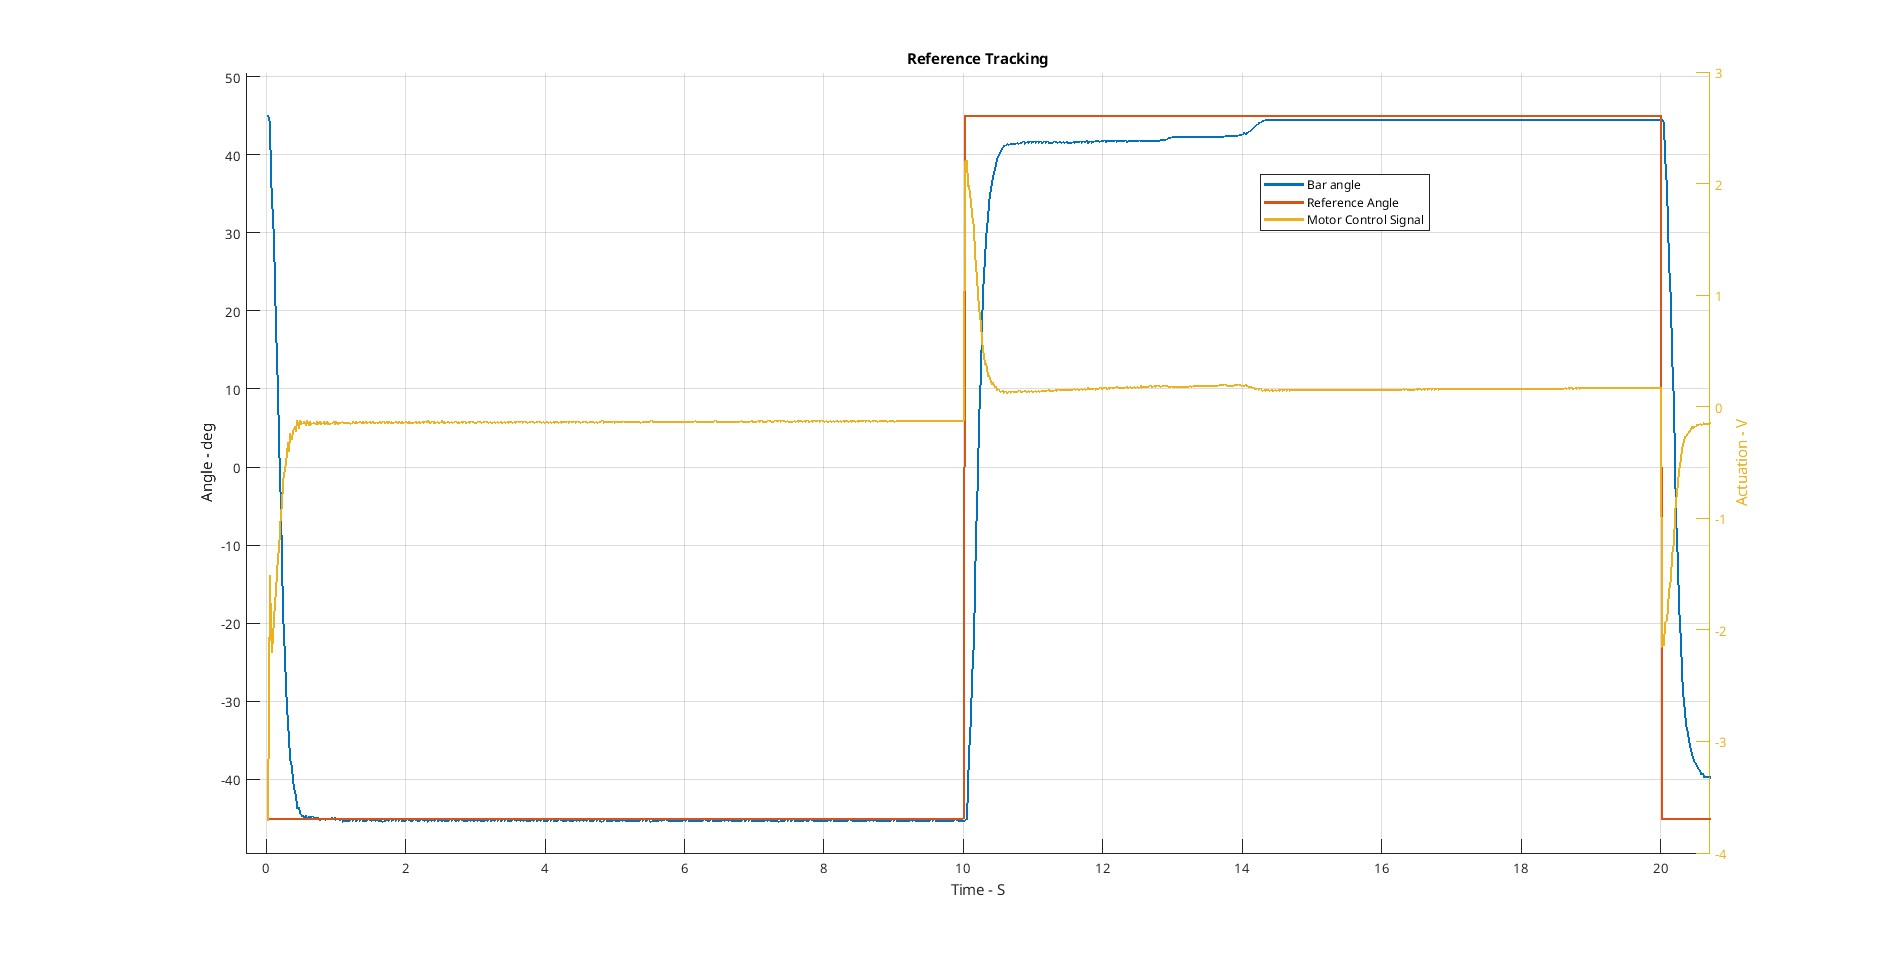
\includegraphics[width=\textwidth]{Figs/Reference Tracking.jpg} 
        \caption{Reference Tracking}
        \label{fig: Reference Tracking} 
    \end{subfigure}
    \hfill
    \begin{subfigure}{0.45\textwidth}
        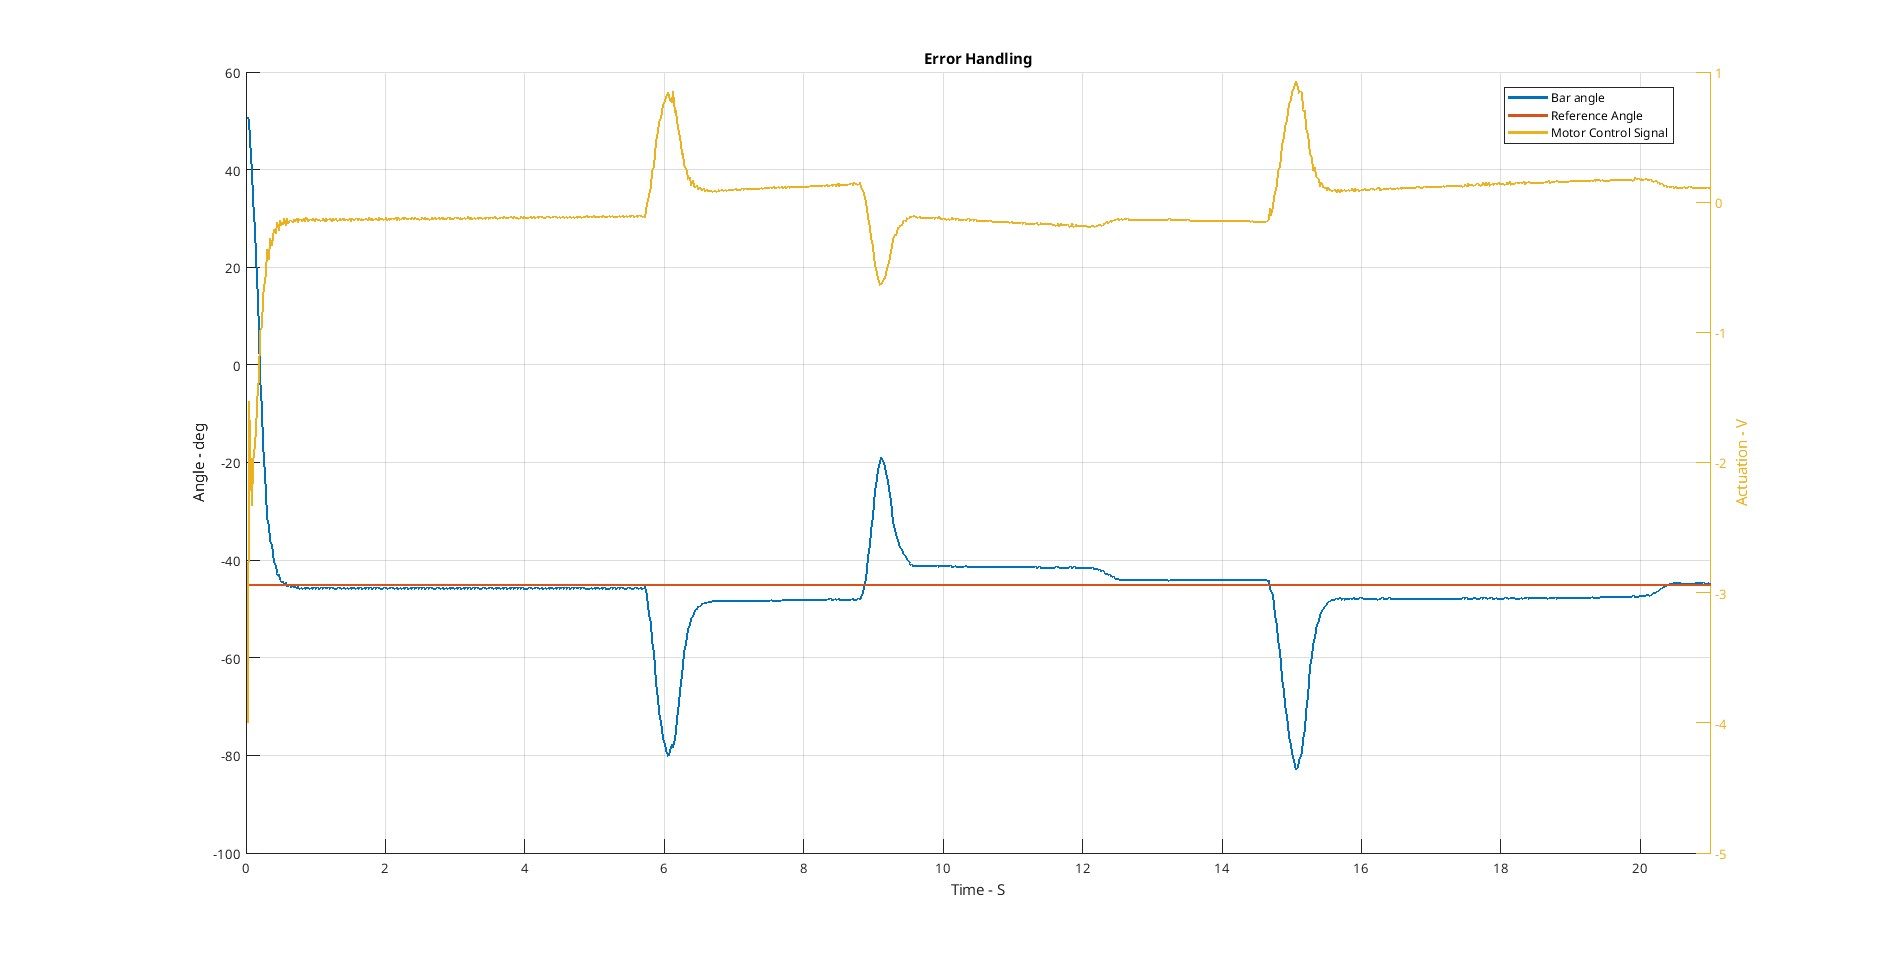
\includegraphics[width=\textwidth]{Figs/Error handling.jpg} 
        \caption{Disturbance handling}
        \label{fig: Disturbance Handling}
    \end{subfigure}
    \caption{Plots showing the performance of the control system}
    \label{fig: Performance Plots}
\end{figure}
